% HUMAN-WRITTEN PART (Andy). This is a DRAFT prepared by the agent from LOG.md, the session transcript, and the
% ShinkaEvolve database; edit freely and verify every claim. Placeholders in [brackets].

\subsection*{2.1 What the autonomous system is}
The research was carried out by two coupled agents. (i) A \emph{research agent}: a Claude Code session (model Claude Fable~5)
driven by the first author's natural-language brief, which surveyed prior work, proposed the three candidate directions,
designed the benchmark (planted-defect classes, witness oracles, generic engine-anomaly oracles, splits), wrote all harness
code (\texttt{autodev/}, \texttt{scripts/}, \texttt{evolve/}), ran and monitored experiments locally and on the UW Hyak cluster,
analyzed results, and wrote Part~1. (ii) A \emph{discovery loop}: ShinkaEvolve~\cite{shinka} evolving a tester program
(\texttt{evolve/initial.py}) with Claude Sonnet~5 as the mutation operator (via the headless CLI provider), fitness computed by
\texttt{autodev/search\_eval.py}. The human's role was to pose the problem, set constraints, approve compute use, and verify.

\subsection*{2.2 Harness and tools}
\textbf{Substrate.} Kinetix 3.0.0 (Jax2D) levels; all levels padded to one static configuration so that batches of levels
run vectorized on one GPU. \textbf{Tester harness} (\texttt{autodev/tester.py}): $B$ workers explore a level for $T$ steps;
$K$ archive slots store full simulator states; a program supplies \texttt{init/restore/act/archive} hooks (pure JAX).
Every first oracle hit records the worker's action buffer and the archive chain back to the level reset, so each reported bug is
re-simulated from reset (\texttt{replay\_chain}) before it is counted. \textbf{Oracles.} Planted classes (OOB, TUNNEL, SHORTCUT,
ANOMALY, DISARMED) with witness predicates on the post-step state; generic engine oracles (left the arena, moving shape inside a
static solid, joint anchors separated, runaway speed / angular velocity / NaN) with per-level thresholds calibrated on random play
and persistence requirements [1,3,2,3 consecutive steps]. \textbf{Design checks}: no-input and random-play outcomes.
\textbf{Compute.} Local CPU (development; discovery-loop fitness for runs 1--3), Hyak A40 GPUs (pool, scans, scaled evaluation; at most 4 GPUs).
From run~4 the fitness itself runs on a GPU: a fitness server (\texttt{scripts/eval\_server.py}) on the cluster scores every candidate the laptop-side
loop ships to it (\texttt{autodev/remote\_eval.py}), so no LLM credentials leave the laptop.


\subsection*{2.3 Prompts and the research loop}
The discovery loop's task prompt (\texttt{evolve/run\_evolution.py}, \texttt{TASK\_SYS\_MSG}) describes the hooks, the fitness,
and the rule that a held-out defect class and held-out levels are excluded from fitness. ShinkaEvolve configuration:
2 islands, archive 30--40, weighted parent selection, \texttt{full}/\texttt{diff} patches, model
\texttt{headless/claude@claude-sonnet-5?effort=medium} (run~1; runs 2--4 add \texttt{claude-opus-5?effort=high}), fitness = mean over search
instances and seeds of $1-\text{steps}/\text{budget}$, budget $64\times1024$ env steps and seeds \{0,1\} (runs 1--3) or $128\times1024$ on the
size-l split with 3 seeds (run~4). All prompts and patches are stored under \texttt{runs/evolve\_*/}. The research
agent's own prompts are the human brief and the session transcript (available on request; excerpts in the appendix).

\subsection*{2.4 Human interventions (ledger excerpt)}
From \texttt{LOG.md}: (1) [Aug 27] posed the problem and asked for three directions. (2) [Aug 28] chose the framing
``bugs found in existing games'', asked for engine and design bugs separately, whole-program search, automatic verification.
(3) [Aug 28--29] set cluster rules (only \texttt{/gscratch/raivn/andy132}, at most half the GPUs, never others' files) and approved
each batch of jobs. (4) [Aug 29, 2:50 AM] open-ended overnight goal (``keep going, look for other methods, use Opus/Sonnet for expensive tasks'').
(5) [Aug 29, morning] reviewed the first results (``72\% is pretty bad''), asked for the methodology, an improvement plan, a survey of other
games and bug-finding benchmarks, and a second proposal with three paths --- the agent's survey then narrowed the paper's novelty claim
(PhyFu already fuzzes Brax) and led to the GPU fitness server. Interventions in the loop itself: the agent stopped run~1 after it
plateaued and restarted from a different seed program (run~2), rotated the held-out class (run~3) and moved fitness to the GPU (run~4);
the human did none of these. The agent made all design decisions listed in 2.2 and the search-space design; the human did not edit
generated programs.

\subsection*{2.5 Verification}
Every number in Part~1 is recomputed by scripts from logs: \texttt{scripts/eval\_baselines.py} (per-instance first-hit arrays,
seeds), \texttt{scripts/report\_bugs.py} (replay-verified anomalies only), \texttt{scripts/figures.py}. Bugs: each flagged state is
re-simulated from reset along its recorded action chain and must re-trigger the oracle; transient one-frame solver hiccups are
excluded by the persistence rule; strips/GIFs are rendered for inspection. Noise: the seed program was re-evaluated on three fresh
seeds (0.593) against the first evolved program (0.620) to establish the fitness noise floor before trusting search gains.
Statistics: 5 seeds per tester and split with 95\% CIs over seeds, plus paired per-instance CIs against the strongest baseline
(the honest one for transfer claims; it includes zero on held-out levels and excludes it on the held-out class). Oracle corrections
found during the run (persistence rule; collision-matrix awareness) are disclosed in Part~1. A third correction came from the
verification step itself: the agent's first bug report described the \texttt{h15\_thrustshoot} anomaly as a block tunnelling through the
ceiling and leaving the arena; replaying the recorded 51-action chain step by step (\texttt{scripts/repro\_h15.py}) showed the block
entering the \emph{right wall's} face at 16.5\,m/s and, in a second chain, the floor, and being ejected within a step --- so the severity
rule was tightened (A only for sustained escapes) and every \texttt{OOB} hit with a 1--2-step duration was re-labelled B. The replay is also a filter, and it caught two harness defects: the per-worker action buffer truncated chains of testers that
never restore, and archive-slot overwrites corrupted the parent pointers of restore-heavy programs (reconstructed chains cycled to
$10^5$ steps). Both were fixed with an append-only lineage log and a buffer flush, verified on planted instances (every chain length
now matches the hit time and all hits replay), and every scan in the paper was re-run with the log; hits from earlier scans are not counted. Prior-art check: an Opus reading
agent re-resolved every citation through the arXiv/GitHub APIs on Aug~29 and found that PhyFu (ASE 2023) already fuzzes Brax with
a penetration oracle; the novelty claim was narrowed accordingly (Part~1, \S1.2).
Known limitations: single game engine; planted classes designed by the agent; the strongest hand-designed baseline
(action-repeat random) was identified only after the search began; the search fitness of runs 1--3 was noisy ($\pm0.02$) and the
search plateaued early; a second engine (Craftax) is planned but not part of this submission. The adaptive portfolio, the
round-2/3 LLM-designed testers, the run-3 (rotated held-out class) candidates and the evolved tester's real-bug scans were still
being evaluated at submission time; the ledger records their status.

\subsection*{2.6 Significance}
% Drafted by the agent from the ledger; edited and approved by the author.
The agent established (i) that a searched tester program transfers to an unseen defect class with a large, instance-significant
gain (0.418 vs.\ 0.266; +0.15 paired), while the gain on unseen levels is modest; (ii) that neither RL testers nor four independent
LLM-designed testers reach it at equal budget; and (iii) a replay-verified list of engine anomalies in shipped and generated Kinetix
levels, of which one shipped-level tunnelling bug is player-triggerable. Without the agent, the human would have built one tester and
one oracle; the benchmark design (planted classes, witness oracles, severity triage, replay verification) and the search were the
agent's. What the agent could not do alone: run the cluster within the lab's rules without guidance, and decide what counts as a
publishable claim.

% Full transfer table (all 15 testers) referenced from Part 1; generated by scripts/make_tables.py.
\input{table_transfer_full.tex}
\input{table_bugs.tex}
\input{table_feasibility.tex}
\begin{figure}[b]\centering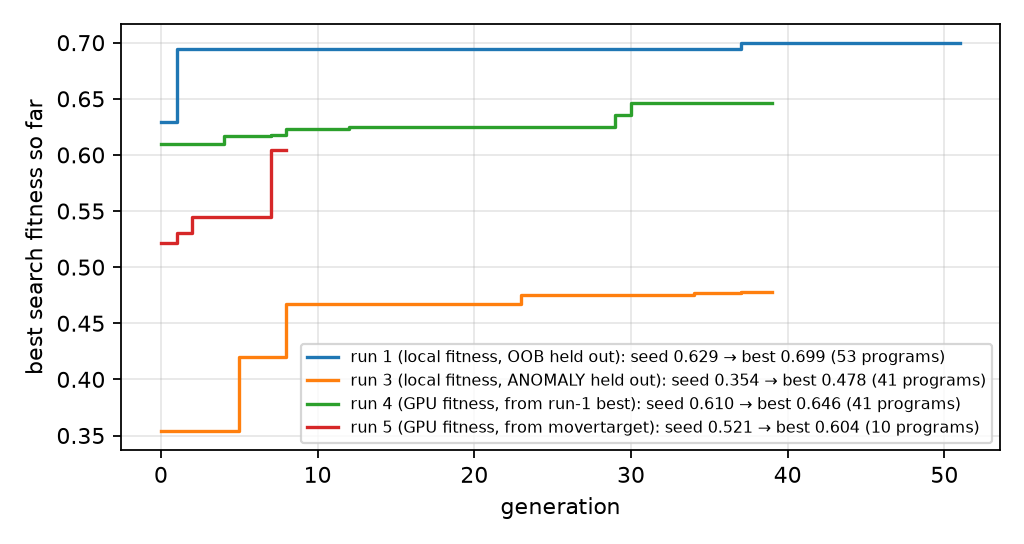
\includegraphics[width=0.52\linewidth]{figures/search_runs.png}
\caption{Best search fitness by generation for the three completed or running searches (each on its own fitness: run 1 and run 3 use the 2-seed local
fitness at $64\times1024$ steps with OOB or ANOMALY held out; run 4 uses the 3-seed GPU fitness on the size-l search split at $128\times1024$,
starting from the run-1 best). Every run makes its largest gain within the first generations and then moves within the noise band.}
\label{fig:fitness}\end{figure}
